%%%%%%%%%%%%%%%%%%%%%%%%%%%%%%%%%%%%%%%%%
% Journal Article
% Advanced Computer Network
% Practical 5: Submit here the topology snap, output of the commands showing the proper configurations of the BGP experiment. Submit your topology file as well. Total two files to be submitted, topology file in GNS3 and output with necessary screens.
%
% Gahan M. Saraiya
% 18MCEC10
%
%%%%%%%%%%%%%%%%%%%%%%%%%%%%%%%%%%%%%%%%%
%----------------------------------------------------------------------------------------
%       PACKAGES AND OTHER DOCUMENT CONFIGURATIONS
%----------------------------------------------------------------------------------------
\documentclass[paper=letter, fontsize=12pt]{article}
\usepackage[english]{babel} % English language/hyphenation
\usepackage{amsmath,amsfonts,amsthm} % Math packages
\usepackage[utf8]{inputenc}
\usepackage{float}

\usepackage{lipsum} % Package to generate dummy text throughout this template
\usepackage{blindtext}
\usepackage{graphicx} 
\usepackage{caption}
\usepackage{subcaption}
\usepackage[sc]{mathpazo} % Use the Palatino font
\usepackage[T1]{fontenc} % Use 8-bit encoding that has 256 glyphs
\usepackage{bbding}  % to use custom itemize font
\linespread{1.05} % Line spacing - Palatino needs more space between lines
\usepackage{microtype} % Slightly tweak font spacing for aesthetics
\usepackage[hmarginratio=1:1,top=32mm,columnsep=20pt]{geometry} % Document margins
\usepackage{multicol} % Used for the two-column layout of the document
%\usepackage[hang, small,labelfont=bf,up,textfont=it,up]{caption} % Custom captions under/above floats in tables or figures
\usepackage{booktabs} % Horizontal rules in tables
\usepackage{float} % Required for tables and figures in the multi-column environment - they need to be placed in specific locations with the [H] (e.g. \begin{table}[H])
\usepackage{hyperref} % For hyperlinks in the PDF
\usepackage{lettrine} % The lettrine is the first enlarged letter at the beginning of the text
\usepackage{paralist} % Used for the compactitem environment which makes bullet points with less space between them
\usepackage{abstract} % Allows abstract customization
\renewcommand{\abstractnamefont}{\normalfont\bfseries} % Set the "Abstract" text to bold
\renewcommand{\abstracttextfont}{\normalfont\small\itshape} % Set the abstract itself to small italic text
\usepackage{titlesec} % Allows customization of titles

\renewcommand\thesection{\Roman{section}} % Roman numerals for the sections
\renewcommand\thesubsection{\Roman{subsection}} % Roman numerals for subsections

\titleformat{\section}[block]{\large\scshape\centering}{\thesection.}{1em}{} % Change the look of the section titles
\titleformat{\subsection}[block]{\large}{\thesubsection.}{1em}{} % Change the look of the section titles
\newcommand{\horrule}[1]{\rule{\linewidth}{#1}} % Create horizontal rule command with 1 argument of height
\usepackage{fancyhdr} % Headers and footers
\pagestyle{fancy} % All pages have headers and footers
\fancyhead{} % Blank out the default header
\fancyfoot{} % Blank out the default footer

\fancyhead[C]{Institute of Technology, Nirma University $\bullet$ October 2018} % Custom header text

\fancyfoot[RO,LE]{\thepage} % Custom footer text
%----------------------------------------------------------------------------------------
%       TITLE SECTION
%----------------------------------------------------------------------------------------
\title{\vspace{-15mm}\fontsize{24pt}{10pt}\selectfont\textbf{Practical 5: BGP Routing Topology}} % Article title
\author{
\large
{\textsc{Gahan Saraiya, 18MCEC10 }}\\[2mm]
%\thanks{A thank you or further information}\\ % Your name
\normalsize \href{mailto:18mcec10@nirmauni.ac.in}{18mcec10@nirmauni.ac.in}\\[2mm] % Your email address
}
\date{}
\hypersetup{
	colorlinks=true,
	linkcolor=blue,
	filecolor=magenta,      
	urlcolor=cyan,
	pdfauthor={Gahan Saraiya},
	pdfcreator={Gahan Saraiya},
	pdfproducer={Gahan Saraiya},
}
%----------------------------------------------------------------------------------------
\usepackage[utf8]{inputenc}
\usepackage[english]{babel}
\usepackage[utf8]{inputenc}
\usepackage{fourier} 
\usepackage{array}
\usepackage{makecell}

\renewcommand\theadalign{bc}
\renewcommand\theadfont{\bfseries}
\renewcommand\theadgape{\Gape[4pt]}
\renewcommand\cellgape{\Gape[4pt]}
\newcommand*\tick{\item[\Checkmark]}
\newcommand*\arrow{\item[$\Rightarrow$]}
\newcommand*\fail{\item[\XSolidBrush]}
\usepackage{xcolor}
\usepackage{minted} % for highlighting code sytax

\definecolor{LightGray}{gray}{0.9}

\setminted[text]{
	baselinestretch=1.2,
	bgcolor=LightGray,
	fontsize=\small
}
\begin{document}
\maketitle % Insert title
\thispagestyle{fancy} % All pages have headers and footers


\section{Introduction}
\paragraph{} Aim of this practical is to create BGP topology in GNS3 according to \href{https://gns3vault.com/bgp/bgp-basic/}{this} link.


\section{Configuration}
Below steps are to be followed in order to initially configure IP address of router.
Here Below are the configuration taken for configuring routers.

\begin{table}[H]
	\centering
	\bgroup
	\setlength{\parindent}{-5em} 
	\caption*{Comparitive analysis}
	\begin{tabular}{r | c | c | c | c }
		\textbf{Router} & \textbf{linked to} & \textbf{Interface} & \textbf{IP address} & \textbf{Subnet}\\
		\hline
		\hline
		R1 (AS 100) & 
		\makecell[l]{
			R2
			\\ R3
		} & 
		\makecell[l]{
			Ethernet 1/1
			\\ Ethernet 1/2
		} & 
		\makecell[l]{
			192.168.12.1
			\\ 192.168.13.1
		} & 
		\makecell[l]{
			255.255.255.0
			\\ 255.255.255.0
		}
		\\
		\hline
		R2 (AS 200) & 
		\makecell[l]{
			R1
		} & 
		\makecell[l]{
			Ethernet 1/1
		} & 
		\makecell[l]{
			192.168.12.2
		} & 
		\makecell[l]{
			255.255.255.0
		}
		\\
		\hline
		R3 (AS 300) & 
		\makecell[l]{
			R1
		} & 
		\makecell[l]{
			Ethernet 1/2
		} & 
		\makecell[l]{
			192.168.13.3
		} & 
		\makecell[l]{
			255.255.255.0
		}
	\end{tabular}
	\egroup
\end{table}

\subsection{Initial Configuration}

\subsubsection{Display interface status in brief}
\begin{minted}{text}
R1#sh ip int br

Interface                  IP-Address      OK? Method Status                Protocol
FastEthernet0/0            unassigned      YES unset  administratively down down
Ethernet1/0                unassigned      YES unset  administratively down down
Ethernet1/1                192.168.12.1    YES manual up                    up
Ethernet1/2                192.168.13.1    YES manual up                    up
Ethernet1/3                unassigned      YES unset  administratively down down
Loopback0                  unassigned      YES unset  up                    up
Loopback1                  unassigned      YES unset  up                    up
Loopback2                  unassigned      YES unset  up                    up
\end{minted}

\subsubsection{Enter to configuration mode}
\begin{minted}{text}
R1#conf t
\end{minted}

\subsubsection{Select interface to work on}
\begin{minted}{text}
R1(config)#int ethernet1/0 
\end{minted}

\subsubsection{Set interface `up` - make active}
\begin{minted}{text}
R1(config-if)#no shut
\end{minted}

\subsubsection{Configure IP address}
\begin{minted}{text}
R1(config-if)#ip address 192.168.12.1 255.255.255.0
\end{minted}

\subsubsection{Setup loopback}
\begin{minted}{text}
R1(config-if)#int loop 0
\end{minted}

\subsection{BGP Configuration of R1}
\begin{minted}{text}

R1(config)#router bgp 100
R1(config-router)#neighbor 192.168.12.2 remote-as 200 
R1(config-router)#
*Nov  4 15:28:21.719: %BGP-5-ADJCHANGE: neighbor 192.168.12.1 Up
R1(config-router)#neighbor 192.168.13.3 remote-as 300 
\end{minted}

\subsubsection{Exiting configuration}
\begin{minted}{text}

R1(config-if)#end
\end{minted}

\subsubsection{Write configuration}
\begin{minted}{text}
R1#wr
\end{minted}

\subsection{Configuration of R2 and R3}
Similarly we will set up router R2 and router R3 with initial configuration following above steps and configure initial configuration.

\subsubsection{R2 IP configuration}
\begin{minted}{text}
R2#sh ip int br
Interface                  IP-Address      OK? Method Status                Protocol
FastEthernet0/0            unassigned      YES NVRAM  administratively down down
FastEthernet0/1            unassigned      YES NVRAM  administratively down down
Ethernet1/0                unassigned      YES NVRAM  administratively down down
Ethernet1/1                192.168.12.2    YES NVRAM  up                    up
Ethernet1/2                unassigned      YES NVRAM  administratively down down
Ethernet1/3                unassigned      YES NVRAM  administratively down down
Loopback0                  2.2.2.2         YES NVRAM  up                    up
\end{minted}

\subsubsection{R3 IP configuration}
\begin{minted}{text}
R3#sh ip int br
Interface                  IP-Address      OK? Method Status                Protocol
FastEthernet0/0            unassigned      YES NVRAM  administratively down down
FastEthernet0/1            unassigned      YES NVRAM  administratively down down
Ethernet1/0                unassigned      YES NVRAM  administratively down down
Ethernet1/1                unassigned      YES NVRAM  administratively down down
Ethernet1/2                192.168.13.3    YES NVRAM  up                    up
Ethernet1/3                unassigned      YES NVRAM  administratively down down
Loopback0                  3.3.3.3         YES NVRAM  up                    up
\end{minted}

\subsection{BGP Configuration}
\subsubsection{R2}
\begin{minted}{text}
R2#conf t
Enter configuration commands, one per line.  End with CNTL/Z.
R2(config)#router bgp 200
R2(config-router)#neighbor 192.168.12.1 remote-as 100
R2(config-router)#end
R2#show ip
*Nov  4 18:45:24.647: %SYS-5-CONFIG_I: Configured from console by console
R2#show ip bgp
\end{minted}

\subsubsection{R3}
\begin{minted}{text}
R3#conf t
Enter configuration commands, one per line.  End with CNTL/Z.
R3(config)#router bgp 300
R3(config-router)#neighbor 192.168.13.1 remote-as 100
R3(config-router)#end
R3#
*Nov  4 18:45:06.015: %SYS-5-CONFIG_I: Configured from console by console
R3#show ip bgp
\end{minted}


\section{Result}
\begin{figure}[H]
	\setlength{\parindent}{-5em}
	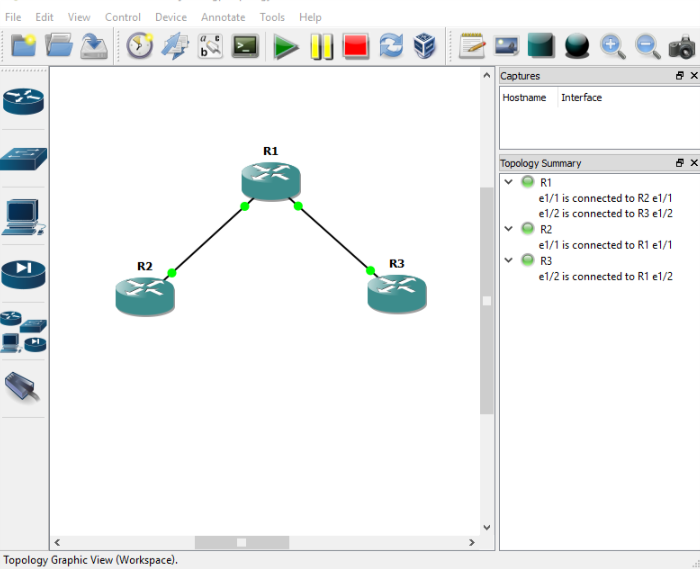
\includegraphics[width=550px]{assets/topology}
	\caption{Topology Summary}
\end{figure}

\begin{figure}[H]
	\setlength{\parindent}{-5em}
	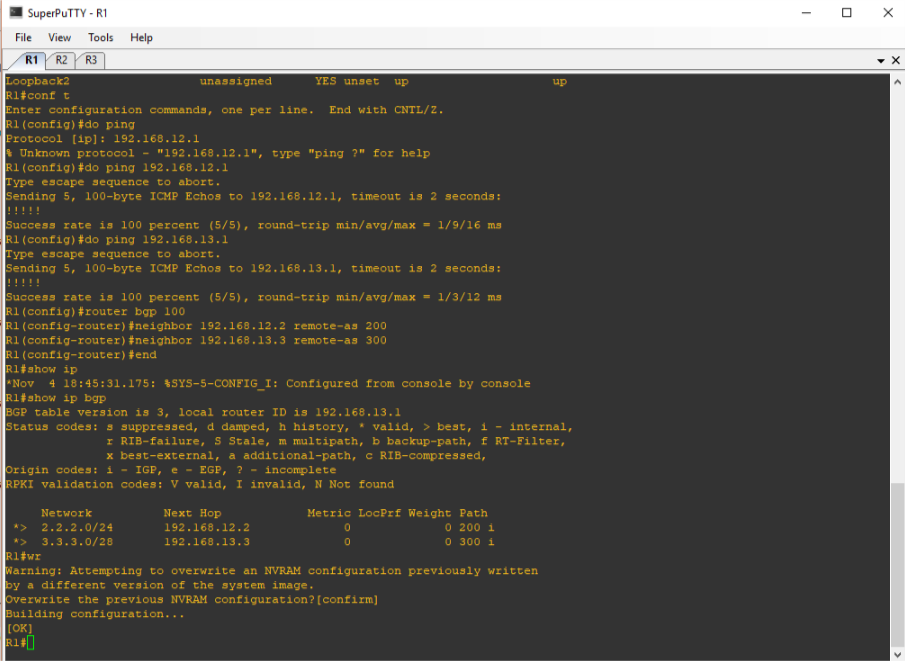
\includegraphics[width=550px]{assets/r1bgp}
	\caption{R1: BGP route status}
\end{figure}

\begin{figure}[H]
	\setlength{\parindent}{-5em}
	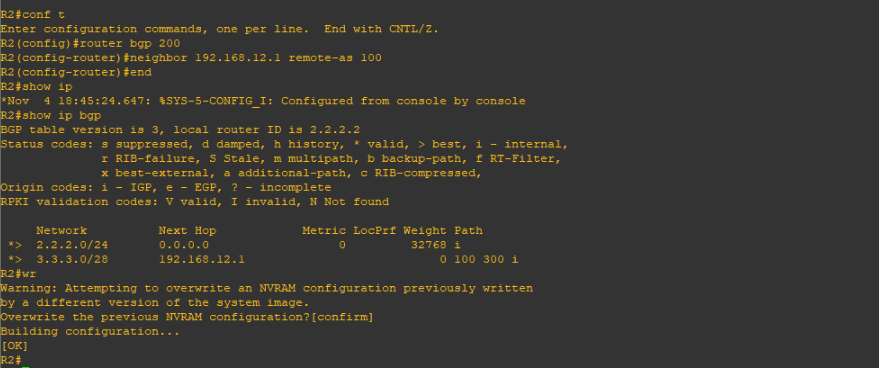
\includegraphics[width=550px]{assets/r2bgp}
	\caption{R2: BGP route status}
\end{figure}

\begin{figure}[H]
	\setlength{\parindent}{-5em}
	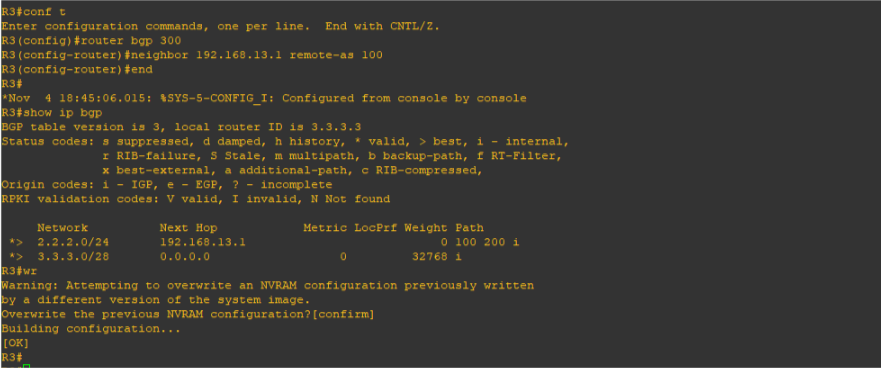
\includegraphics[width=550px]{assets/r3bgp}
	\caption{R3: BGP route status}
\end{figure}



\end{document}
